Bremsstrahlung photons emitted by beam halo muons in the ECAL volume generate a physical EM shower in the ECAL crystals~\cite{Halo2015}. 
Large energy deposits are rare, but the rate of beam halo penetration during the 2016 run was substantial.
The characteristic features of a shower caused by a halo particle include coincident hits in the barrel muon system and a ``trail'' of low-energy clusters in ECAL along the particle trajectory. 
The beam halo MET filter described in Section~\ref{sec:pf_met} exploits the former, while the \emip\ variable described in Section~\ref{sec:pf_photons} captures the latter.

\begin{figure}[htbp]
  \centering
  \resizebox{\textwidth}{!}{
    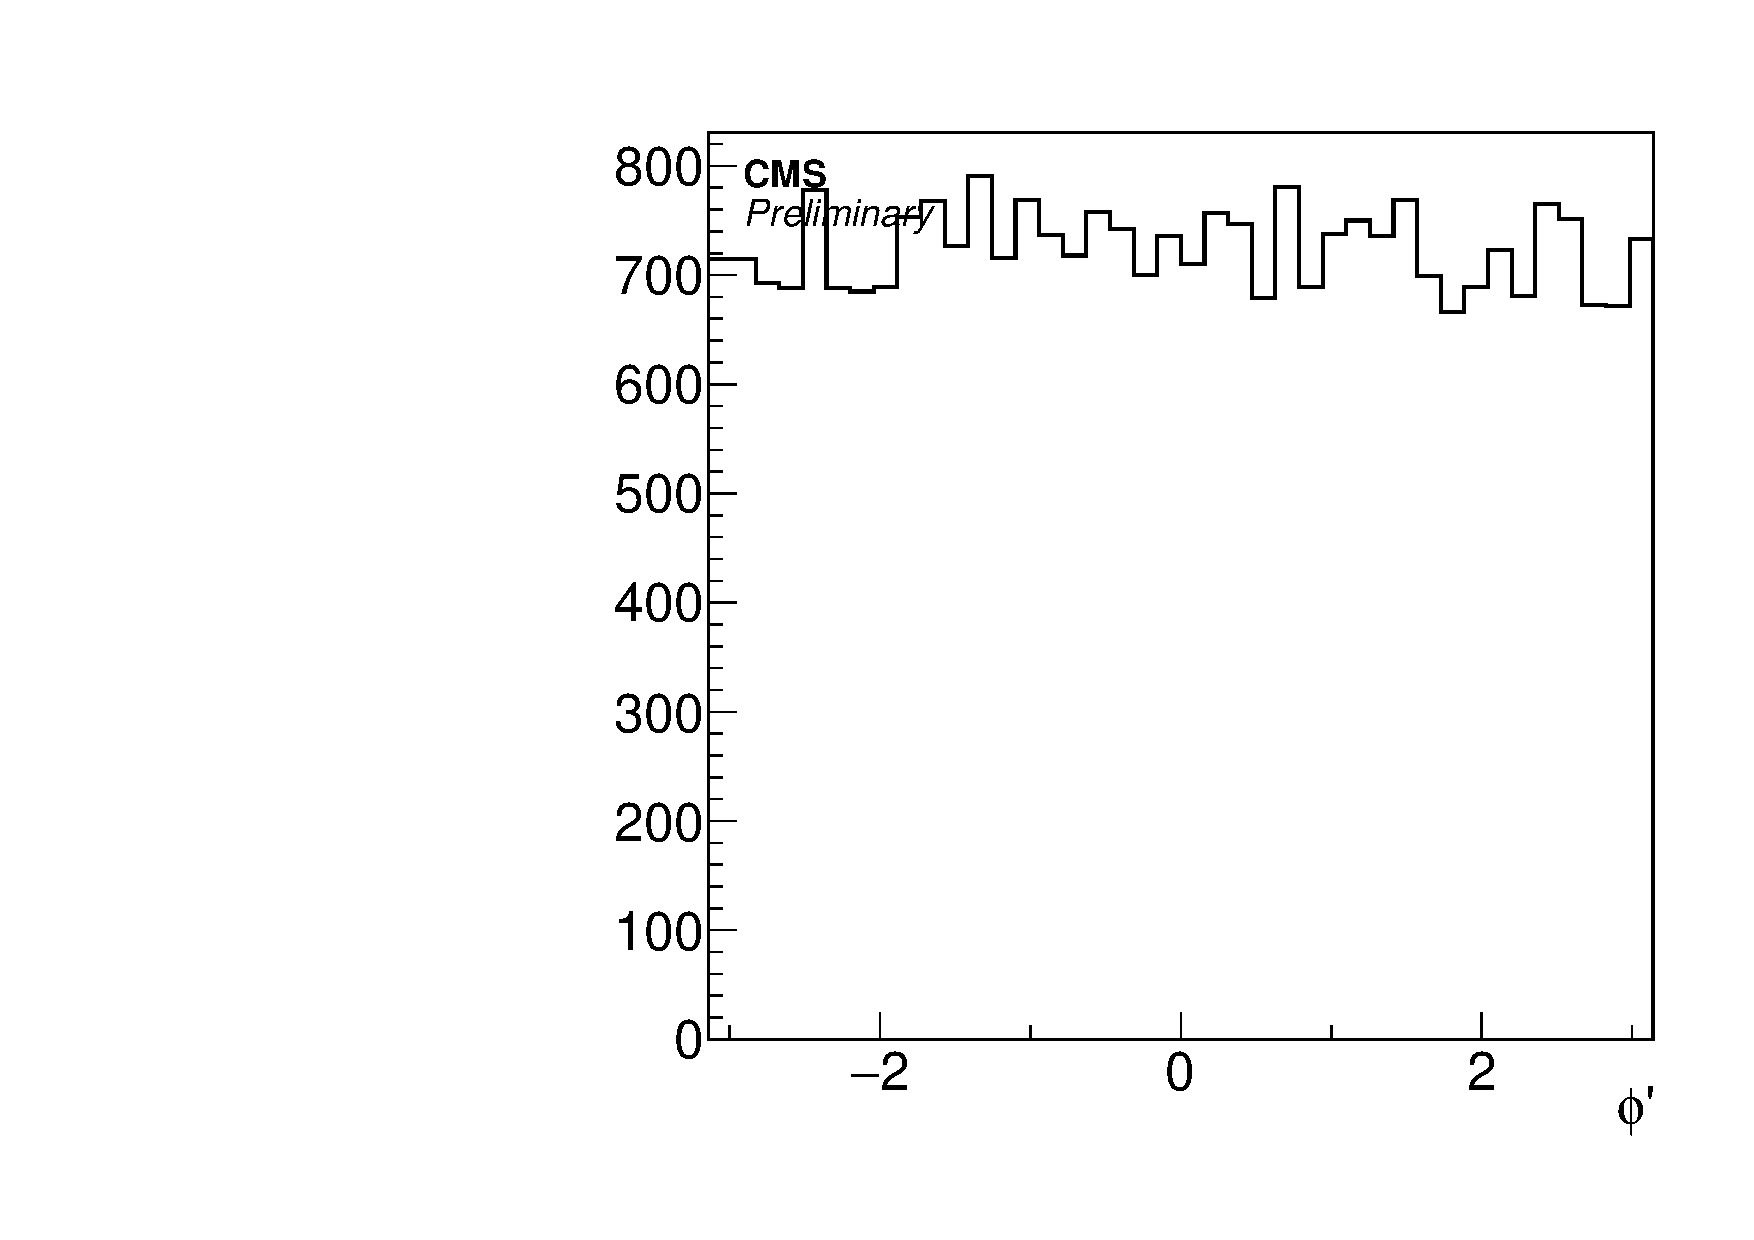
\includegraphics[]{Reconstruction/Figures/halo/bkgphi.pdf}
    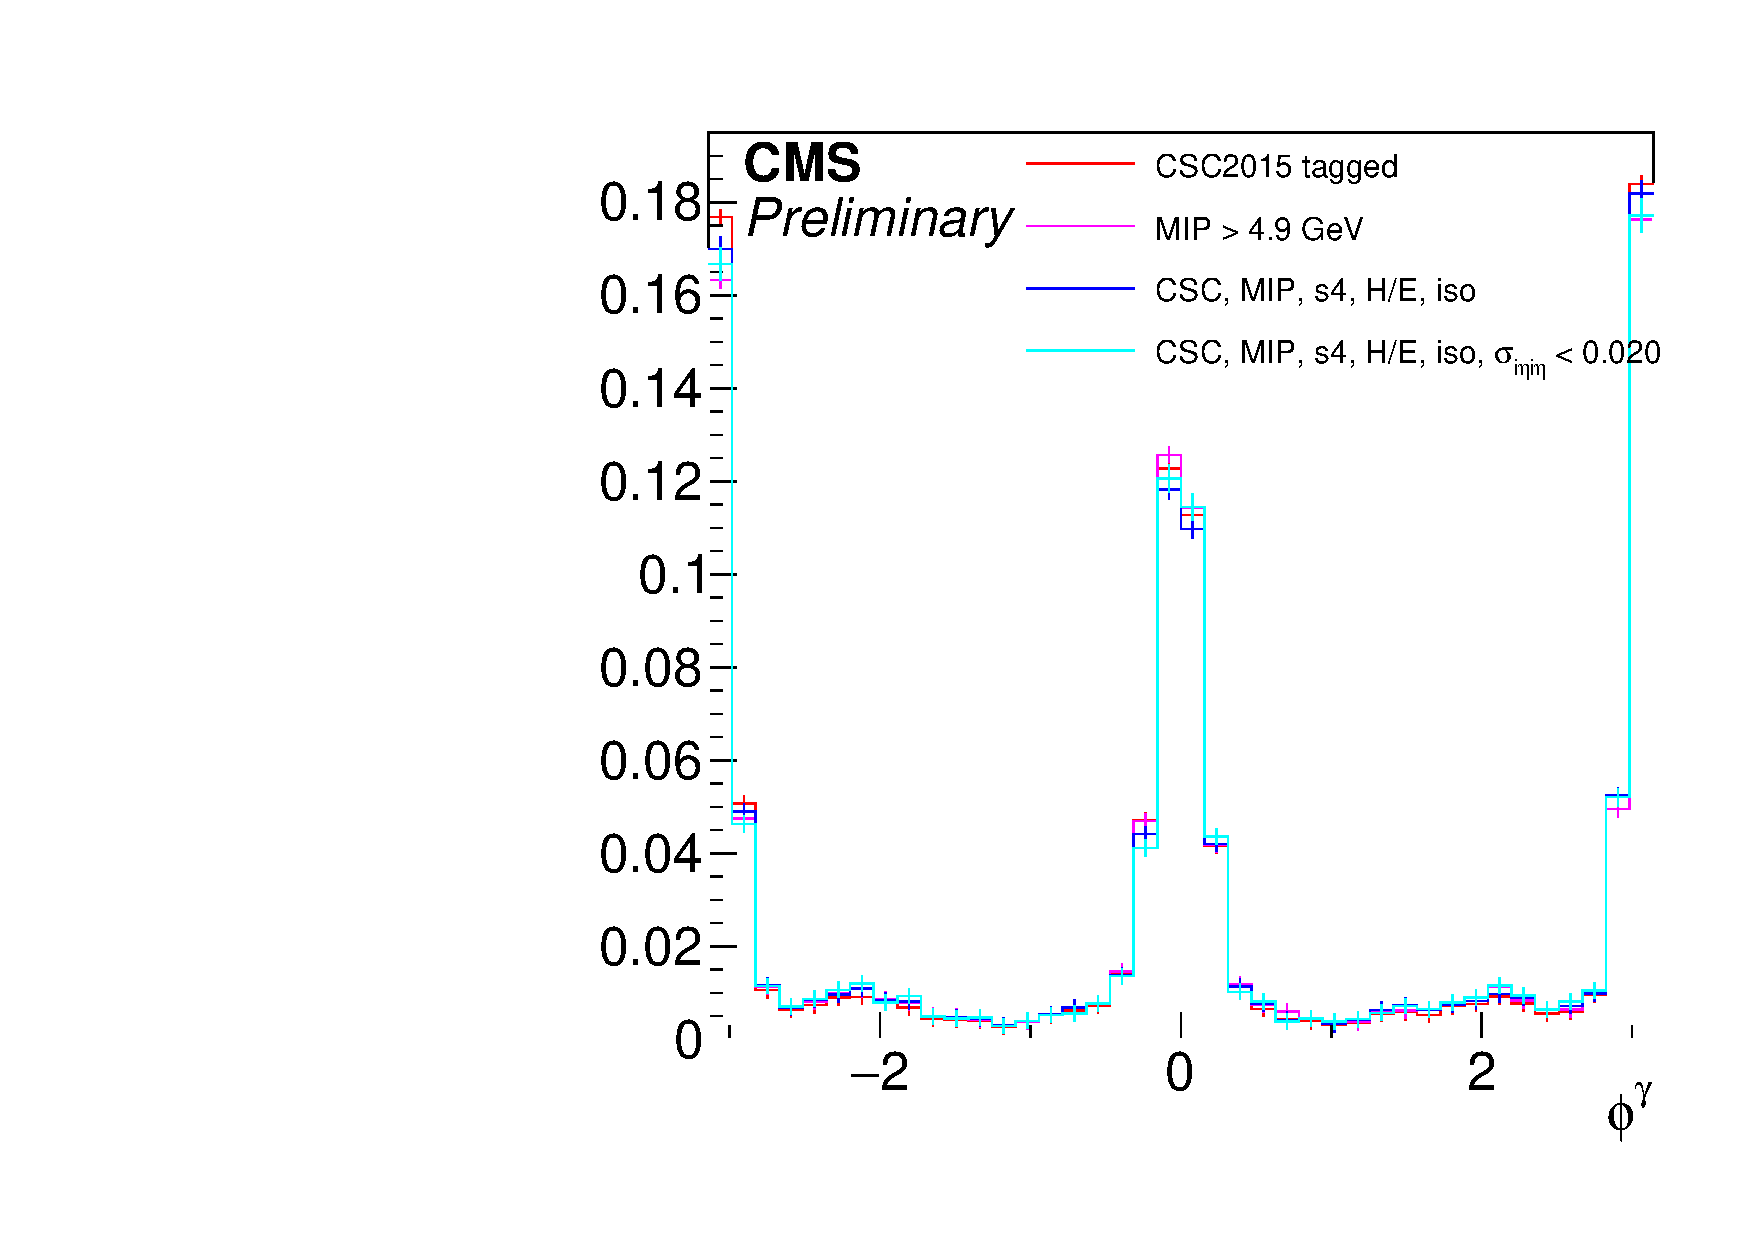
\includegraphics[]{Reconstruction/Figures/halo/halophi.pdf}
  }
  \caption{
    Left: The \phig\ distribution from \zinvg\ MC simulation. \qquad \qquad
    Right: The \phig\ distribution of the halo-like showers, tagged either by the CSC halo filter or that fail the MIP-tagging.
    Histograms are normalized to unity.
    The cyan histogram is the \phig\ distribution after applying photon identification selections except for the shower shape. 
    It can be seen that the \phig\ distribution is highly stable against the listed identification selections.
  }
  \label{fig:halophi}
\end{figure}

Because beam halo particles are produced through complex LHC machine effects, the observed distribution of the halo showers is not
symmetric in the azimuthal angle in the detector coordinates.
The right side of Figure~\ref{fig:halophi} is a \phig\ distribution of the halo showers obtained from the SinglePhoton dataset, requiring $\met > 140\GeV$. 
Halo showers are defined as those that fail the MIP-tagging of $\emip < 4.9$ and those in events tagged by the CSC beam halo tagger.
On the other hand, reconstructed showers from all other sources are symmetric in \phig\, as shown on the left side of Figure~\ref{fig:halophi}. 

\begin{figure}[htbp]
  \centering
  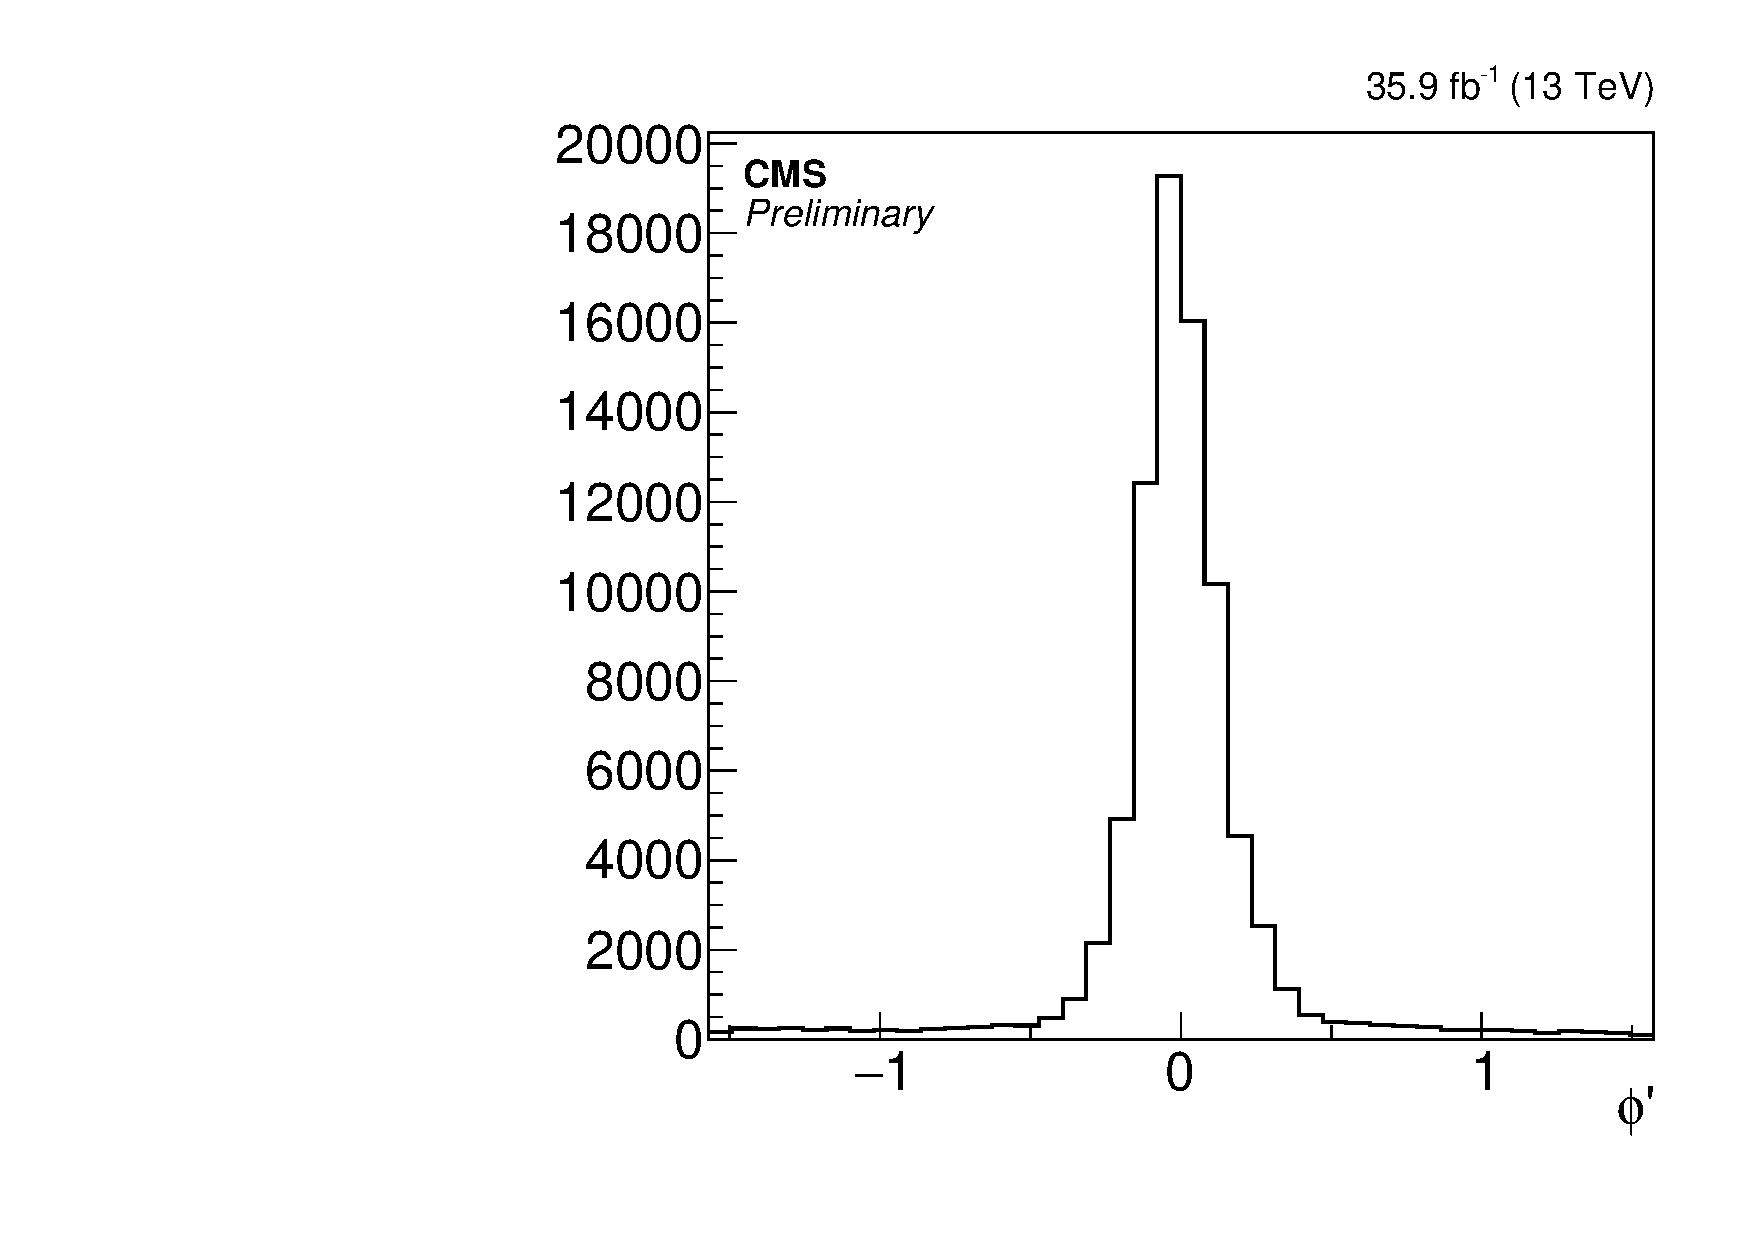
\includegraphics[width=0.5\textwidth]{Reconstruction/Figures/halo/haloPhiFolded.pdf}
  \caption{
    Folded $\phi'$ distribution of the halo sample.
  }
  \label{fig:halo_template}
\end{figure}

To ensure that the the distribution of Fig.~\ref{fig:halophi} is a valid template for halo showers and invariant under photon selection requirements, the \phig\ distribution is folded such that the two peaks of the halo showers coincide.
To match the positions of the peaks in the halo template, the distribution is shifted by 0.005 and then folded along 0. 
The new angular variable $\phi'$
\begin{equation}
  \phi' := \left|\left[\left[\phig + 0.005\right]_{-\pi}^{\pi} - \frac{\pi}{2}\right]_{-\pi}^{\pi}\right| - \frac{\pi}{2},
  \label{eqn:phi}
\end{equation}
where $[\cdot]_{\pi}^{\pi}$ signifies casting the content into range $[-\pi,\pi]$,
exhibits a unimodal distribution for the halo template, as shown in Fig.~\ref{fig:halo_template}.

\begin{figure}[htbp]
  \centering
  \resizebox{\textwidth}{!}{
    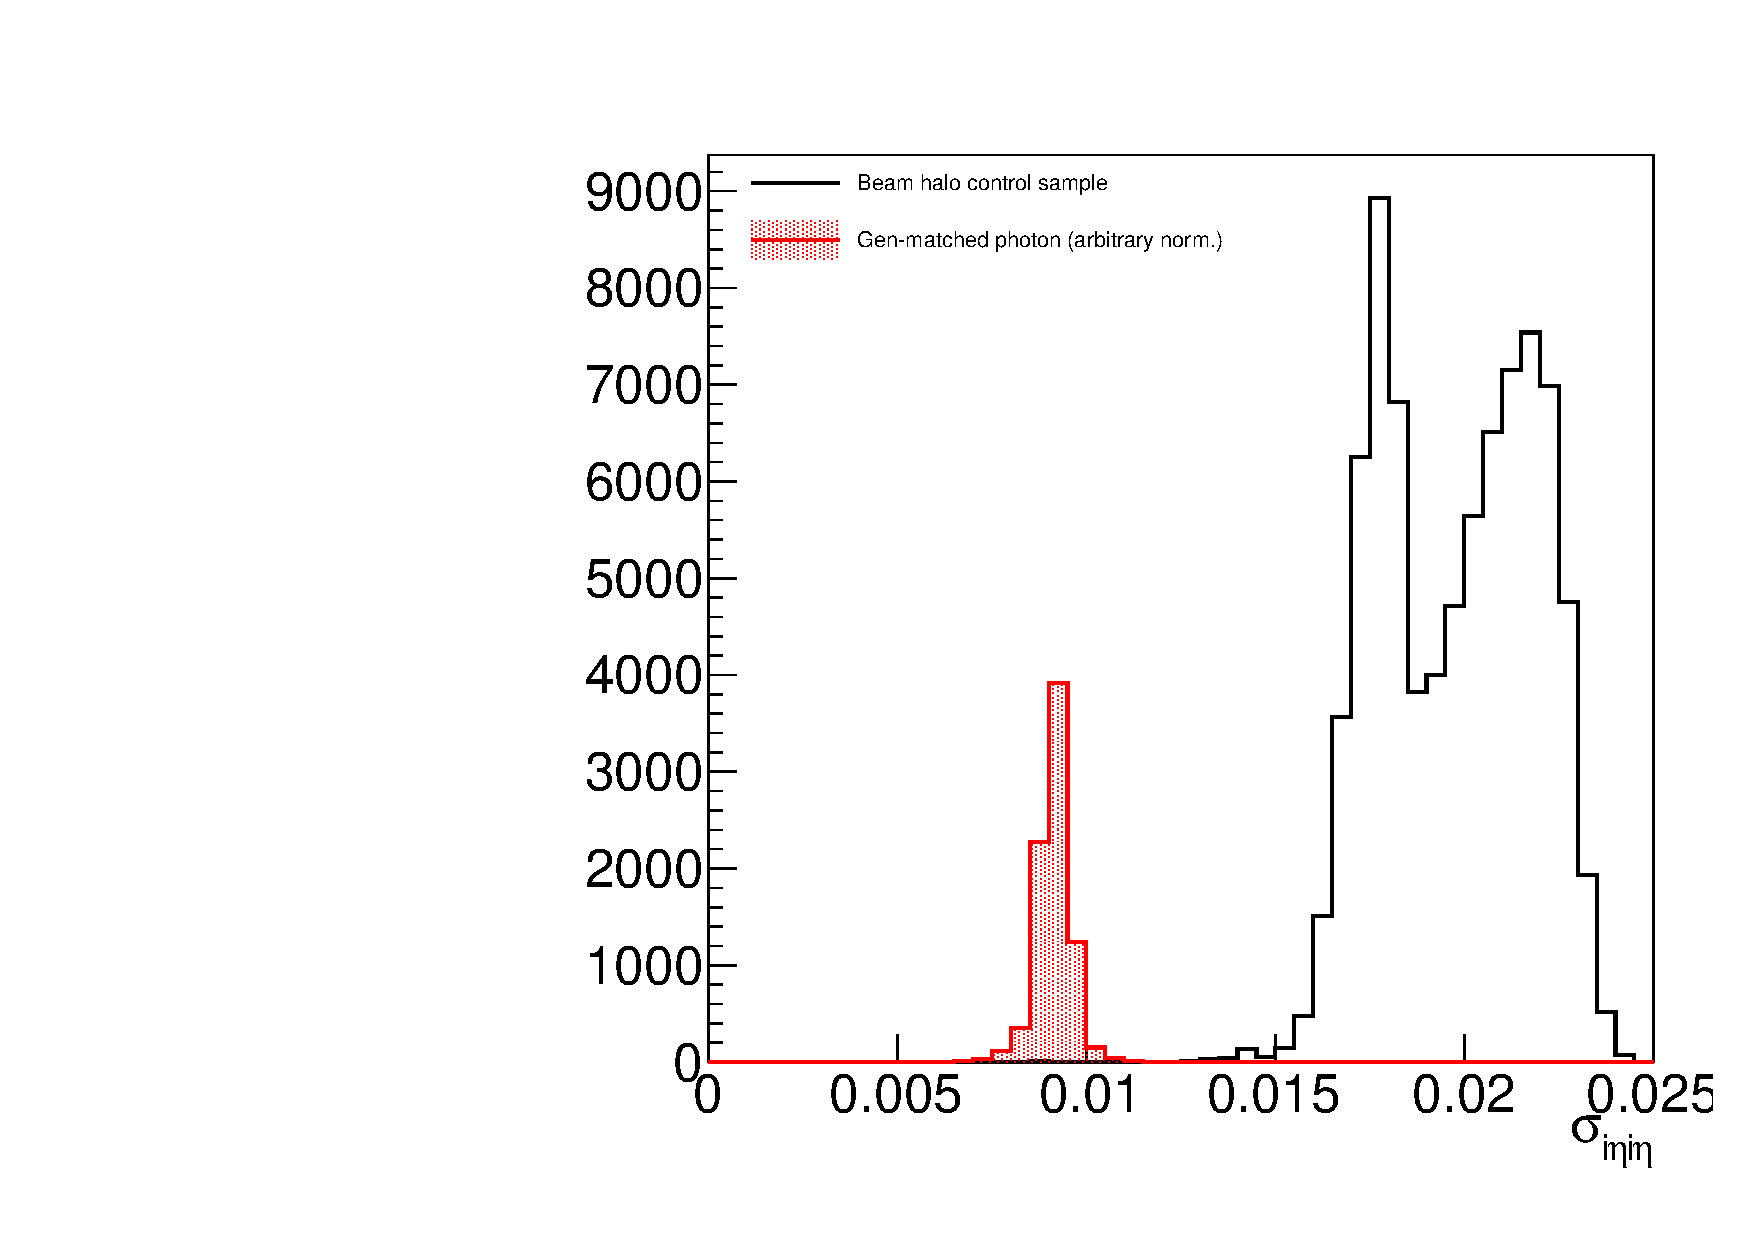
\includegraphics[]{Reconstruction/Figures/halo/halo_sieie.pdf}
    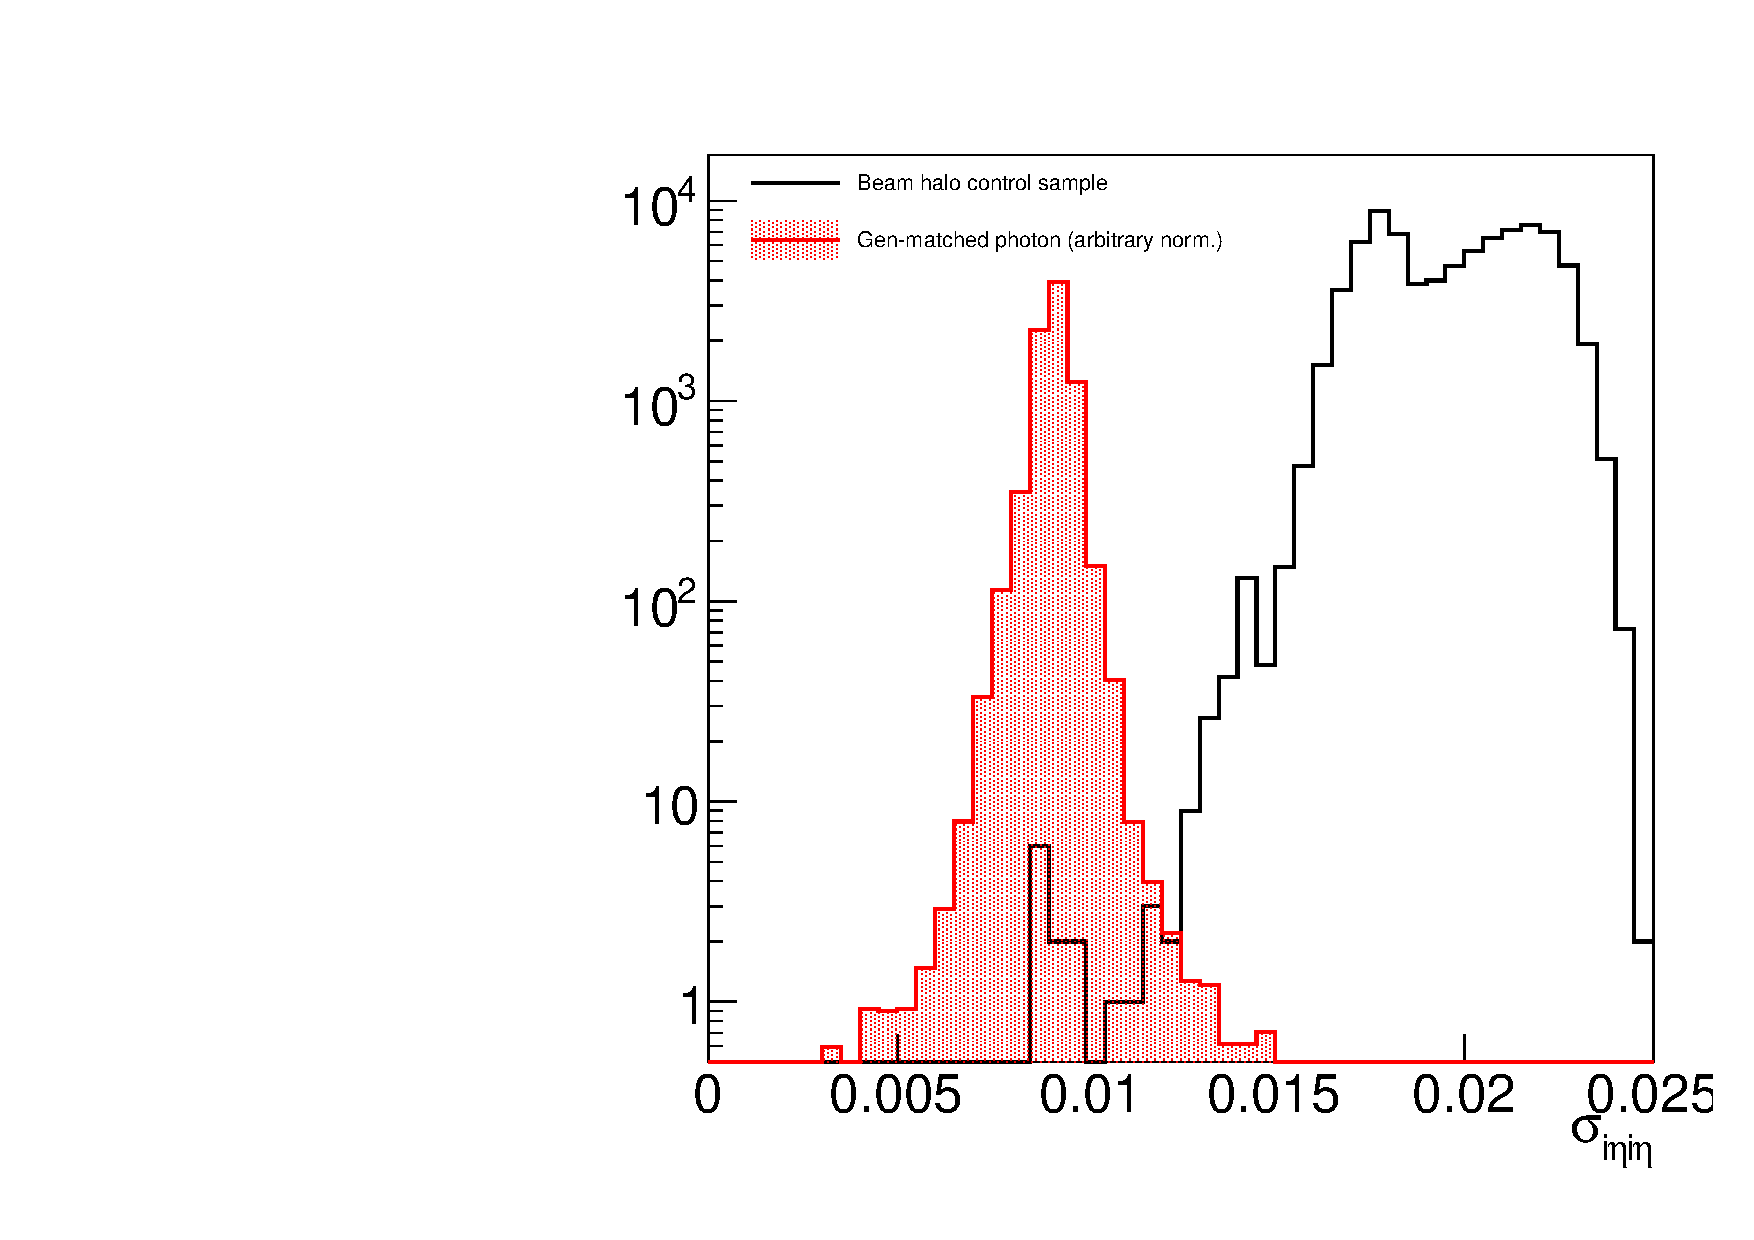
\includegraphics[]{Reconstruction/Figures/halo/halo_sieie_log.pdf}
  }
  \caption{
    The \sieie distribution of the beam halo control sample and a reference distribution from truth-matched MC photons. 
    Left: linear scale, Right: log scale. 
    There is a small peak at $\sieie \sim 0.01$ in the beam halo control sample, which is not visible in linear-scale.
  }
  \label{fig:halo_sieie}
\end{figure}

The contribution of real photons into the halo control sample is negligible.
This is confirmed from the \sieie\ distribution of the halo control sample and the correlation between \sieie\ and \emip\ in a MC true-photon sample.
The \sieie\ distribution of the halo control sample features a small peak at $\sieie \sim 0.01$, which can be attributed to contributions from true photons, as the photon \sieie distribution overlaid in Figure~\ref{fig:halo_sieie} suggests. 
However, the contribution of true photons diminishes rapidly with increasing \sieie. 
Additionally, Figure~\ref{fig:sieie_mip_corr} illustrates that the shape of the true-photon \sieie\ does not change significantly with respect to \emip. 
From these two observations, we can see that there are is only a negligible number of true photons in the halo control sample.

\begin{figure}[htbp]
  \centering
  \resizebox{0.45\textwidth}{!}{
    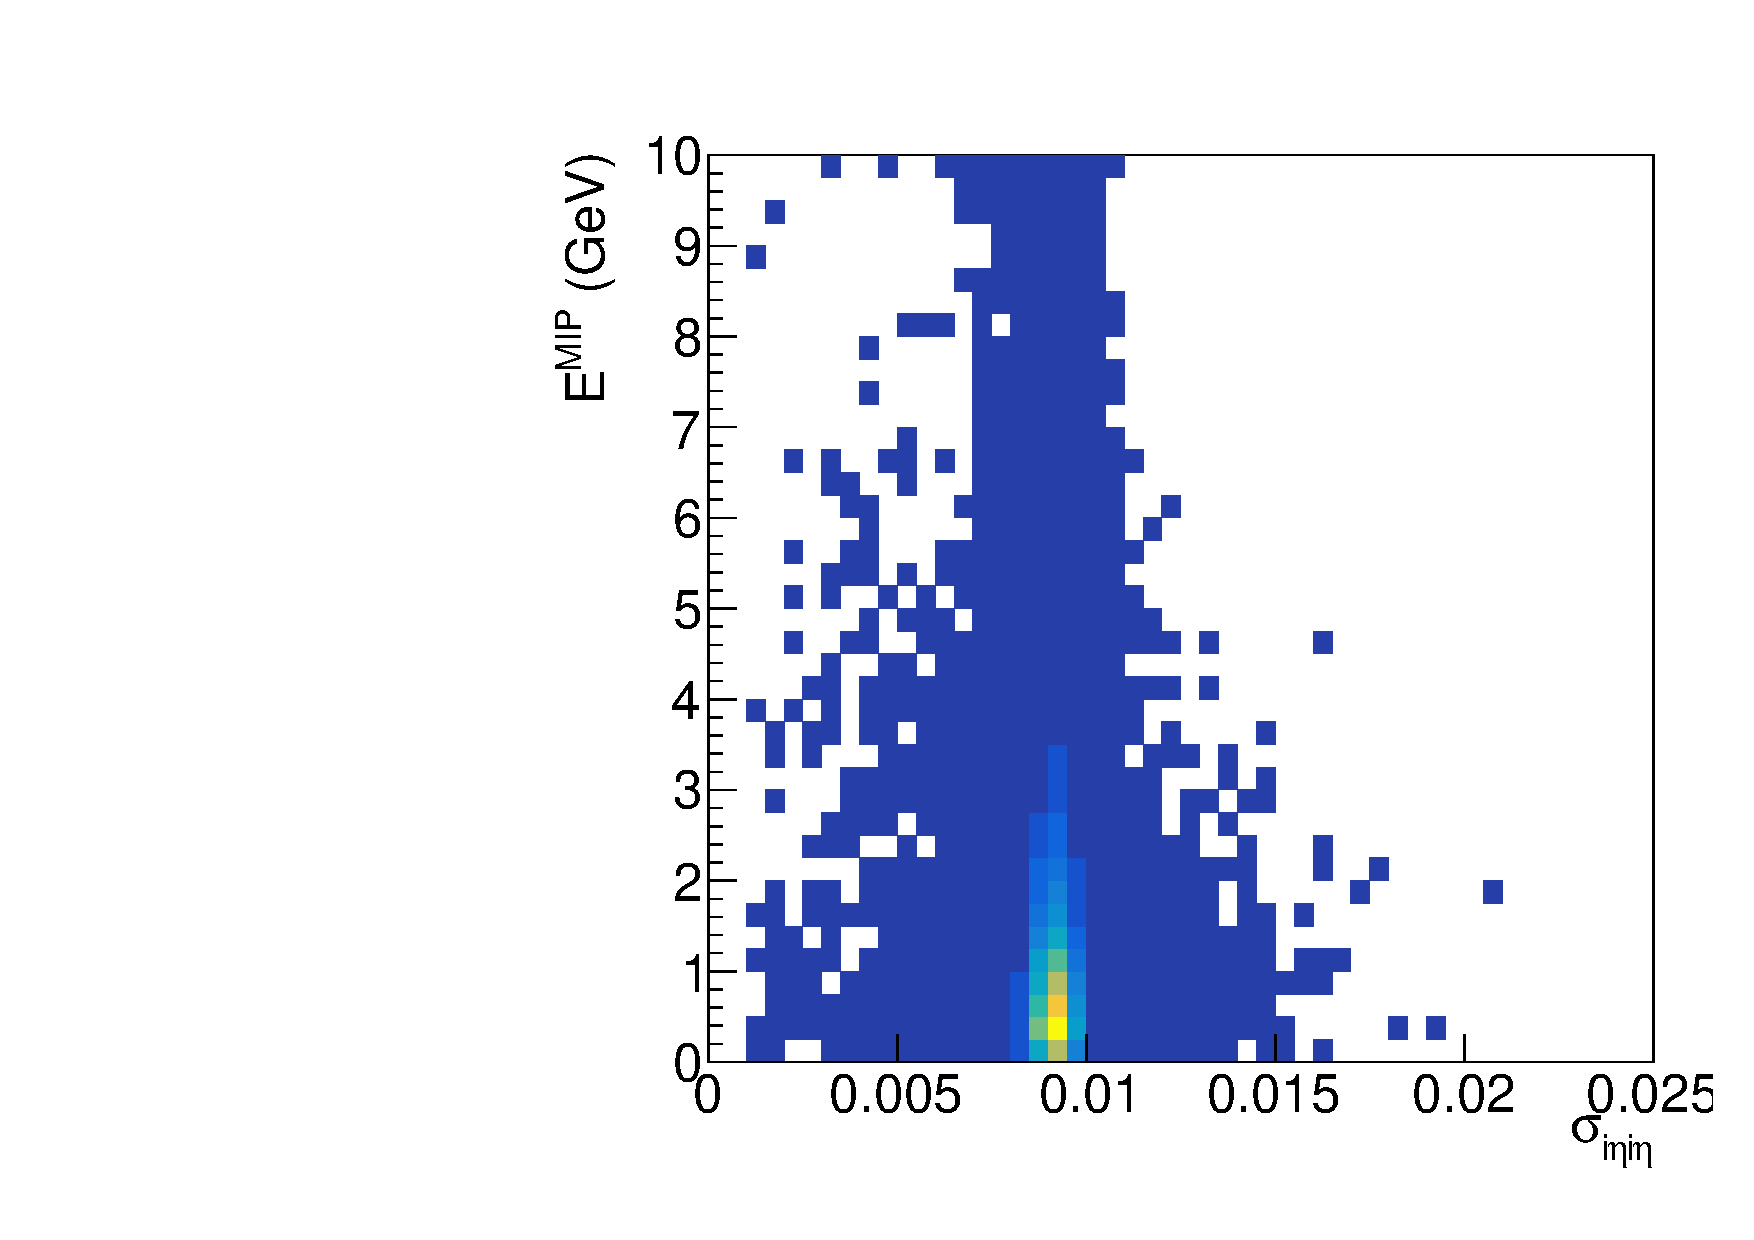
\includegraphics[]{Reconstruction/Figures/halo/sieie_mip_corr.pdf}
  }
  \caption{
    Correlation between \sieie\ and \emip\ in truth-matched MC photons. 
  }
  \label{fig:sieie_mip_corr}
\end{figure}

While the peaking behavior is a robust feature of the halo showers, their rate is not easily predictable. 
Therefore,  a two-template fit to the $\phi'$ distribution of the photons in the candidate sample, where the templates are a uniform distribution (Figure~\ref{fig:halophi} left) and that of the halo shower (Figure~\ref{fig:halo_template}), accurately estimates the amount of beam halo background present in the signal region.

For this analysis, the two-template fit is replicated by splitting the signal region into two parts according to the variable $\phi'$ introduced in Equation~\ref{eqn:phi}.
This enables us to determine the beam halo contribution during the signal extraction procedure.
The region defined by $\abs{\phi'} < 0.5$ is called the horizontal ($H$) region, its complement $0.5 < \abs{\phi'} < \pi/2$ is called the vertical ($V$) region.
A schematic of these regions is shown in Figure~\ref{fig:split_diagram}.

\begin{figure}[htbp]
  \centering
  \resizebox{0.75\textwidth}{!}{
    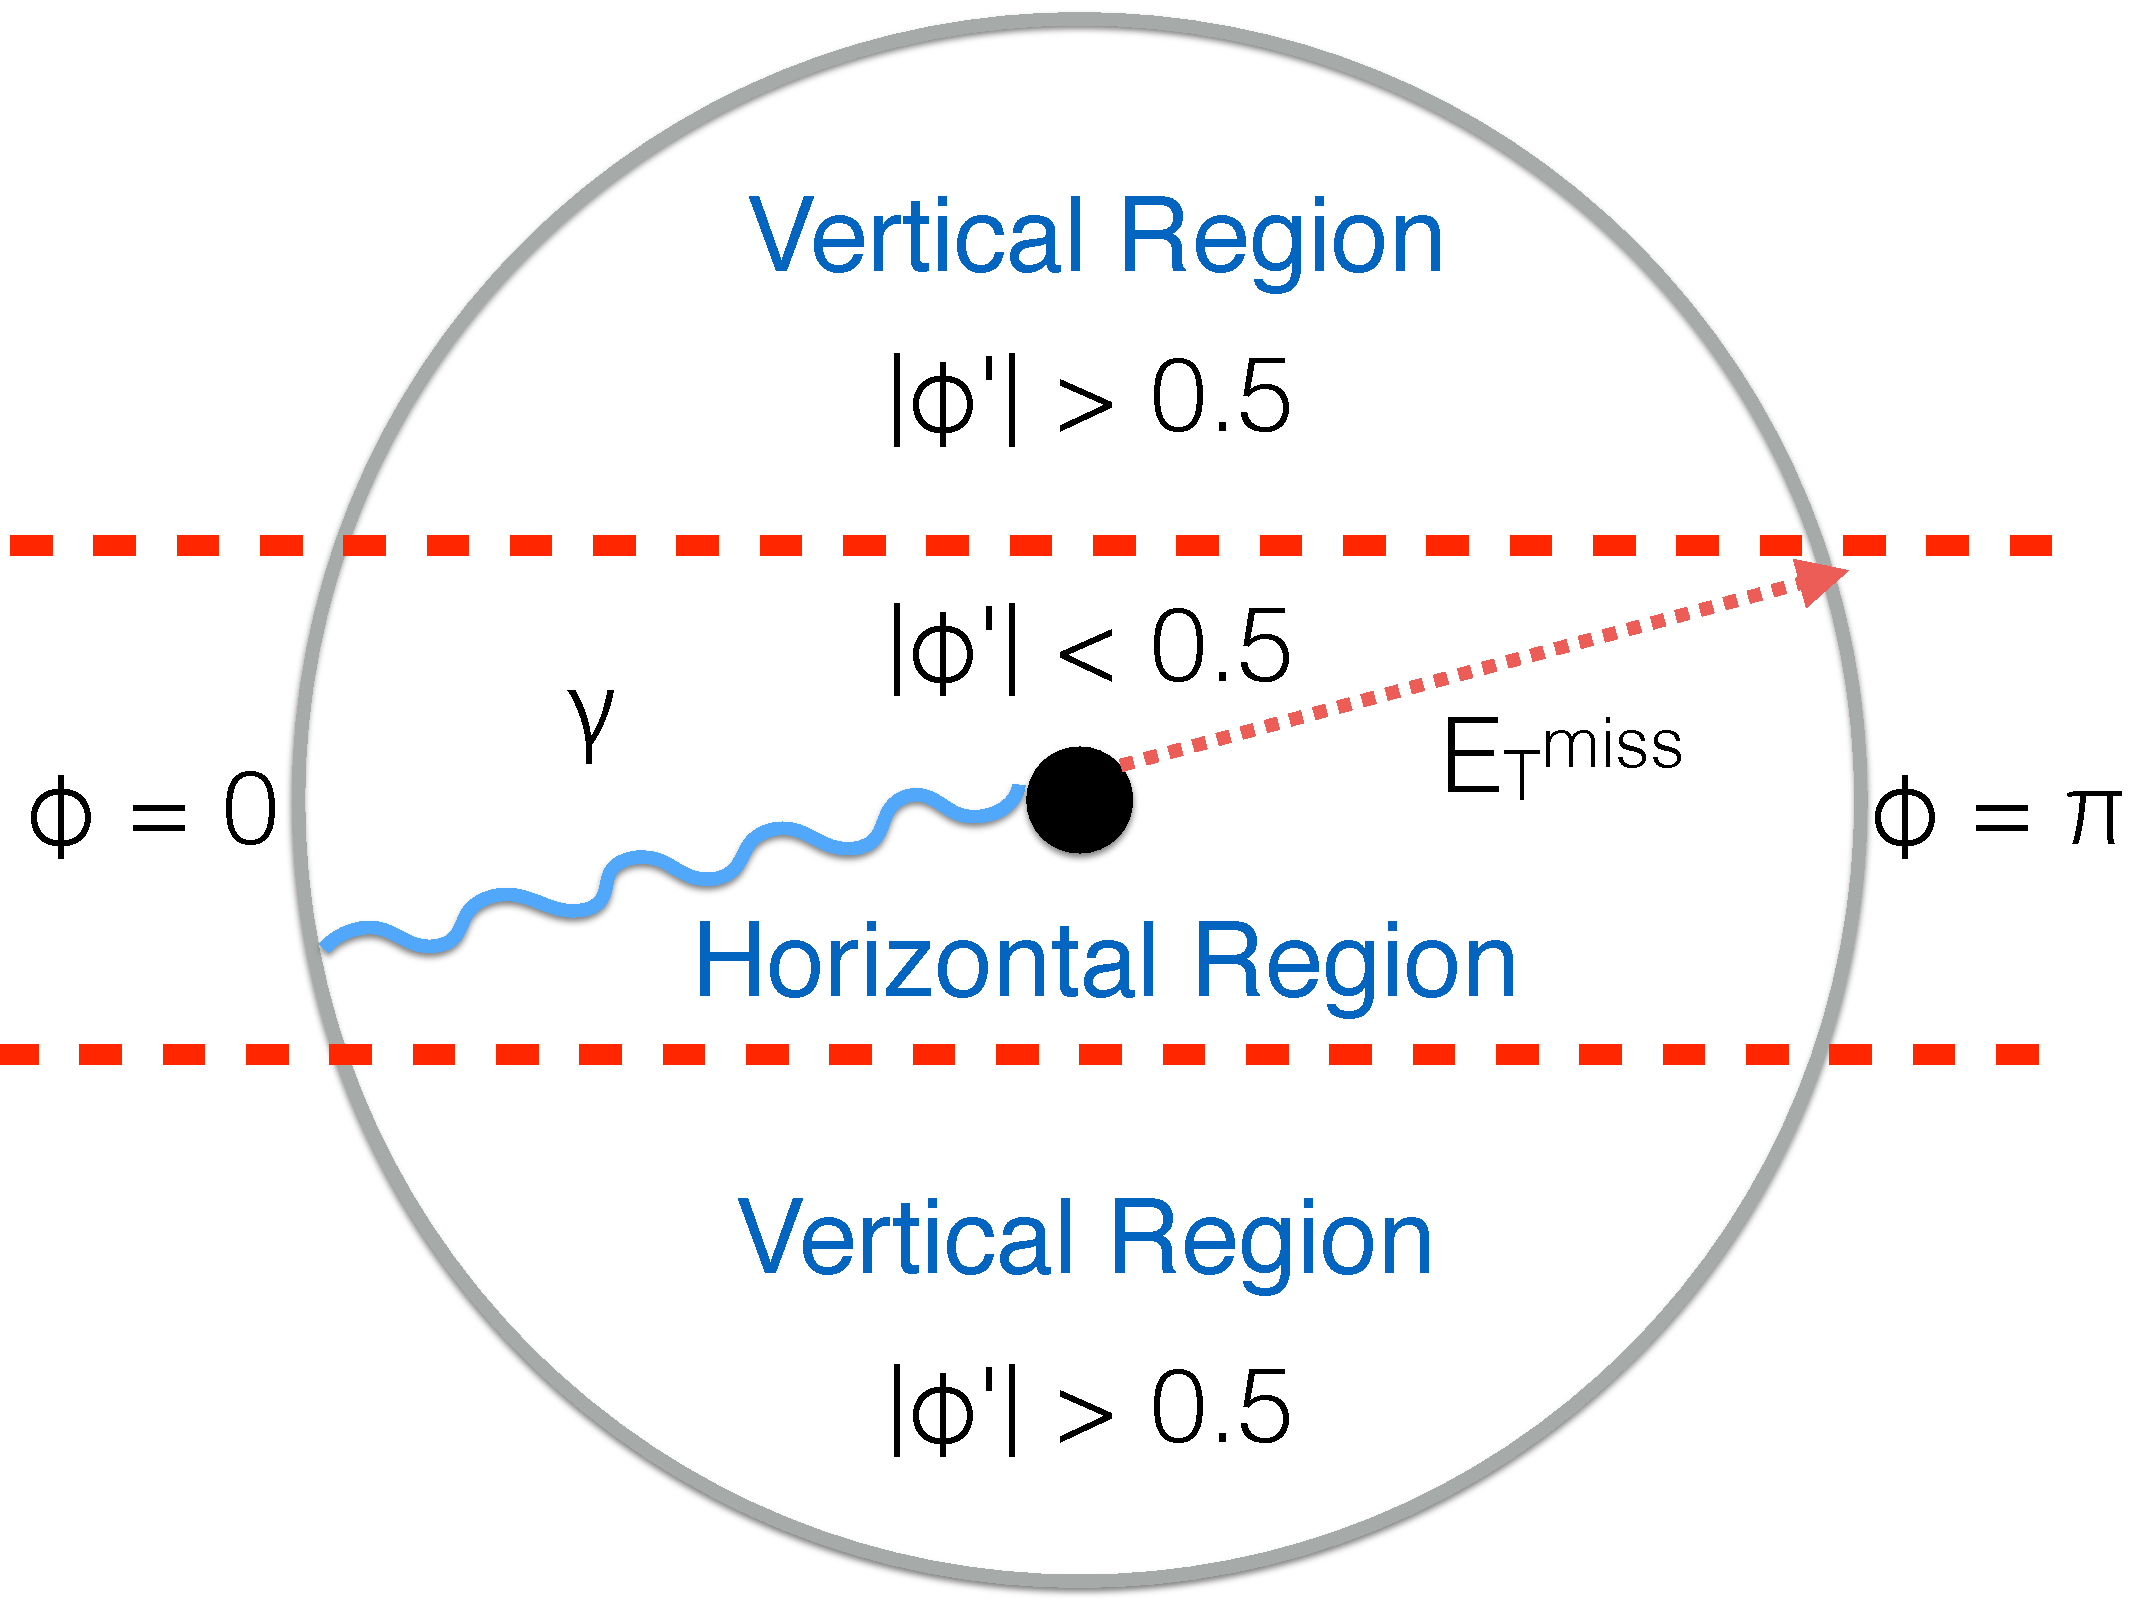
\includegraphics[]{Analysis/Figures/split_diagram.pdf}
  }
  \caption{
        Schematic of splitting the signal region into horizontal and vertical regions.
        The red lines are a rough demarcation of the split; they do not represent the exact line $\abs{\phi'} = 0.5$.
        A sample beam halo event with a photon and \met\ is shown for reference.
      }
    \label{fig:split_diagram}
\end{figure}

In the horizontal and vertical signal regions, collision processes occupy the relative fractions of phase space $C_{H} = 1/\pi$ and $C_{V} = (\pi-1)/\pi$, respesctively. 
% corresponding to $\abs{\phi'} < 0.5$ and $0.5 < \abs{\phi'} < \pi/2$
The corresponding fractions for beam halo events are determined by selecting a halo-enriched sample where the halo veto is inverted. 
Thus, a fit of the two signal regions provides an estimate of the overall normalization of the beam halo background, denoted $h$.
 
The \ETg\ dependence of the halo background is encoded in \nhalo[,i], the unit-normalized beam halo prediction in the $i^\mathrm{th}$ bin of the signal region $K \in \{H,V\}$.
Using the notation introduced in Section~\ref{sec:irreducible}, the total estimated background \TK\ in the two signal regions are
\begin{equation}
\begin{aligned}
  \TK[,i] & = C_{K} \left( \NZg[i] + \NWg[i] + b_{K,i}\right) + h \nhalo[,i]  \\
          & = C_{K} \left( \left[1 + \left(\fZW[,i]\right)^{-1}\right] \NZg[i] + b_{K,i}\right) + h \nhalo[,i],
\end{aligned}
\end{equation}
where $b_{K,i}$ is the total contribution to bin $i$ of region $K$ from electron and hadron misidentification, ECAL spikes, and other minor SM background processes.

